\documentclass[tikz, border=2mm]{standalone}
\usetikzlibrary{intersections, angles, quotes}

\begin{document}
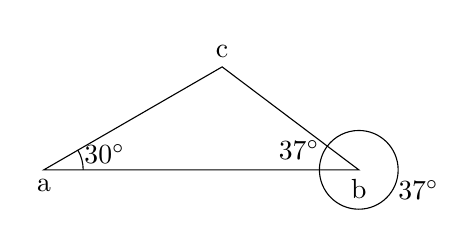
\begin{tikzpicture}
\draw coordinate[label=below:a] (a) --++(0:4cm) coordinate[label=below:b] (b);

\path[name path=ac] (a)--++(30:3cm);
\path[name path=bc] (b)--++(180-37:3cm);

\path [name intersections={of = ac and bc, by=c}];

\node[above] at (c) {c};

\draw[use as bounding box] (a)--(b)--(c)--cycle%
     pic[draw, "$30^\circ$", angle eccentricity=1.6] {angle=b--a--c}
    pic[draw, "$37^\circ$", angle eccentricity=1.6] {angle=c--b--a}
    pic[draw, "$37^\circ$", angle eccentricity=1.6] {angle=a--b--c};
\end{tikzpicture}
\end{document}